\chapter{Processi e Metodi}
\label{cap:processi-metodologie}

\indent Questo capitolo fornisce in dettaglio l'ambiente di ricerca utilizzato, le tecnologie impiegate e descrive gli esperimenti condotti. 
Provvede a dare inoltre tutte le informazioni necessarie per replicare gli esperimenti.

\section{Ambiente}  
~\\  
\indent In questa sezione vengono descritti gli strumenti utilizzati durante il progetto, con le relative versioni riassunte nella Tabella \ref{table-tecnologie}.  
\\  
L'intero progetto è stato sviluppato su \textbf{\emph{MacOS}}\footnote{\url{https://support.apple.com/en-us/111893}}. La scelta di questo sistema operativo è stata motivata dalla familiarità con l'ecosistema Apple e dalle elevate prestazioni del processore, oltre che dalla vasta disponibilità di strumenti per l'analisi e lo sviluppo.  
\\  
Per la decompilazione degli eseguibili è stato utilizzato \textbf{\emph{Ghidra}}\footnote{\url{https://ghidra-sre.org/}}, uno strumento open source per l'ingegneria inversa, sviluppato dalla NSA's Research Directorate. La scelta è ricaduta su questo software poiché è open source e già noto al tirocinante.  
\\  
Il codice è stato condiviso e mantenuto tramite \textbf{GitHub}\footnote{\url{https://github.com/}}.  
\\  
Per la realizzazione degli esperimenti, il linguaggio di programmazione principale impiegato è stato \textbf{Python}\footnote{\url{https://python.org/}}. Python è stato scelto per la sua versatilità e l'ampia disponibilità di librerie, che hanno facilitato lo sviluppo rapido di prototipi e script.  
\\  
Per la classificazione delle sottofamiglie di malware è stato utilizzato \textbf{AVClass2}\footnote{\url{https://github.com/malicialab/avclass}}, un tool open source sviluppato da MaliciaLab, che consente di classificare i campioni di malware in base a famiglia e sottofamiglia partendo da report in formato JSON.  
\\  
I campioni di malware sono stati scaricati da tre fonti affidabili e riconosciute: \textbf{Malshare}\footnote{\url{https://malshare.com/pull.php}}, \textbf{Malware Bazaar}\footnote{\url{https://bazaar.abuse.ch/}} e \textbf{VirusShare}\footnote{\url{https://virusshare.com/}}.  
\\  
Per la generazione dei report relativi a ciascun malware è stato utilizzato \textbf{VirusTotal}\footnote{\url{https://www.virustotal.com/}}, un servizio online di scansione antivirus che analizza file e URL per rilevare malware e fornire dettagli sulle minacce.  
\\  
Infine, per determinare la presenza di un packer in un malware, è stato impiegato \textbf{Detect it Easy (DiE)}\footnote{\url{https://github.com/horsicq/Detect-It-Easy}}, uno strumento popolare tra analisti di malware, esperti di cybersecurity e reverse engineer. DiE supporta l'analisi sia basata su firme che euristica, ed è compatibile con una vasta gamma di piattaforme, come Windows, Linux e MacOS. Grazie alla sua architettura adattabile e basata su script, DiE si distingue come uno degli strumenti più versatili nel settore.

\hfill
\begin{table}[!h]
    \centering
    \begin{tabular}{|c|c|c|}
        \hline
        \textbf{Tipo} & \textbf{Nome} & \textbf{Versione} \\
        \hline
        Applicativo & \emph{Chromium} & 131.0.6778.70 \\
        \hline
        Applicativo & \emph{Ghidra} & 11.1.2 \\
        \hline
        Applicativo & \emph{Git} & 2.46.0 \\
        \hline
        Applicativo & \emph{Github} & Versione attuale \\
        \hline
        Applicativo & \emph{AVClass2} & Versione attuale \\
        \hline
        Applicativo & \emph{DiE} & Versione attuale \\
        \hline
        Applicativo & \emph{Visual Studio Code} & 1.95.3 \\
        \hline
        Sistema Operativo & \emph{MacOS} & Sonoma 14.6 \\
        \hline
        Linguaggio & \emph{Python} & 3.13.0 \\
        \hline
    \end{tabular}
    \vspace*{.2cm}
    \caption{Tabella riassuntiva tecnologie usate}
    \label{table-tecnologie}
\end{table}

\subsection{Svolgimento del Progetto}
Il progetto è stato sviluppato attraverso una serie di fasi distinte, ciascuna delle quali ha contribuito alla creazione di un sistema per l'analisi e la generazione di malware. Le fasi sono state le seguenti:
\begin{enumerate}
    \item \textbf{Ricerca, raccolta e classificazione dei dati}: In questa fase iniziale, è stata condotta una ricerca approfondita per reperire dataset contenenti campioni di malware. I dati sono stati raccolti da fonti affidabili e riconosciute nel settore, tra cui \textbf{VirusShare}, \textbf{MalwareBazaar} e \textbf{Malshare}, utilizzando le risorse messe a disposizione da queste piattaforme per il download di campioni di malware. Una volta ottenuti i campioni, è stato utilizzato \textbf{VirusTotal} per generare i report di analisi di ciascun campione. Successivamente, i malware sono stati classificati nelle rispettive famiglie tramite l'uso dello strumento \textbf{AVClass2}, che ha permesso di ottenere una classificazione precisa dei campioni in base alle loro caratteristiche. Una volta ottenuto il dataset di malware classificati, si è proceduto con la fase successiva.
    
    \item \textbf{Preprocessing}: Durante questa fase, i malware sono stati disassemblati per estrarre il loro codice esadecimale e assembly. In particolare, dall'assembly si è scelto di considerare solo le istruzioni mnemoniche, ignorando qualsiasi altro tipo di dato. Questi mnemonici rappresentano le operazioni fondamentali svolte dal codice, fornendo una sintesi compatta e significativa del comportamento del malware. Dopo aver estratto i mnemonici, si sono generate tutte le possibili coppie di mnemonici, cioè sequenze di due istruzioni consecutive, per catturare le relazioni immediate tra le operazioni eseguite.
    Una volta ottenute le coppie di mnemonici, si è applicata la tecnica TF-IDF (Term Frequency - Inverse Document Frequency), che consente di quantificare l'importanza di ciascuna coppia nel contesto dell'intero dataset. L'uso di TF-IDF permette di ridurre l'influenza di coppie di mnemonici troppo comuni (meno informative) e di enfatizzare quelle che risultano particolarmente distintive per certe famiglie di malware. Successivamente, è stata applicata la \textbf{PCA} (Principal Component Analysis), che ha permesso di ridurre la dimensionalità dei dati e identificare le coppie di istruzioni mnemoniche che avevano il maggior impatto nella classificazione. Questo processo ha facilitato la pulizia dei dati, eliminando informazioni non rilevanti e il rumore che altrimenti avrebbe disturbato l'analisi delle caratteristiche.
    Dai componenti principali ottenuti, si è generata una matrice di dimensione 16x16, che rappresenta una sorta di "impronta" del comportamento del malware. Questa matrice è stata poi normalizzata utilizzando la tecnica Min-Max Scaling, che trasforma i valori della matrice in un range tra 0 e 255, permettendo così di rappresentarli come intensità di pixel.
    La formula applicata è riportata di seguito:
    \[
    M'_{ij} = \frac{M_{ij} - \min(M)}{\max(M) - \min(M)} \times (255 - 0) + 0
    \]

    Dove:
    \begin{itemize}
    \item \( M_{ij} \) è il valore del componente principale nella posizione \( (i, j) \) della matrice originale.
    \item \( \min(M) \) e \( \max(M) \) sono rispettivamente il valore minimo e massimo della matrice \( M \).
    \item \( M'_{ij} \) è il valore normalizzato della matrice, scalato nel range \( [0, 255] \), che corrisponde all'intensità di un pixel nell'immagine finale.
    \end{itemize}
    Infine, la matrice normalizzata è stata convertita in un'immagine in scala di grigi, dove ogni pixel rappresenta un valore numerico della matrice scalato tra 0 (nero) e 255 (bianco). Queste immagini sono state poi utilizzate come input per il modello di rete neurale convoluzionale.

    \item \textbf{Addestramento}: Durante questa fase, è stata progettata e addestrata una rete neurale convoluzionale (CNN) per la classificazione dei malware. Il modello è stato ottimizzato per riconoscere le diverse superfamiglie di malware a partire dalle immagini generate durante il preprocessing. Il dataset è stato suddiviso in tre set: l'80\% dei campioni è stato utilizzato per l'addestramento, il 10\% per il test e il restante 10\% per la validazione. La struttura del modello comprende sequenzialmente: due strati convoluzionali con 64 filtri ciascuno, seguiti da strati di max pooling; un terzo strato convoluzionale anch'esso seguito da max pooling; infine, una sequenza di strati fully connected, compresi uno strato Flatten e due strati Dense, con un layer Dropout tra di loro per ridurre il rischio di overfitting. L'addestramento è stato eseguito utilizzando un approccio di apprendimento supervisionato, impiegando diverse tecniche di regolarizzazione e ottimizzazione degli iperparametri per migliorare le prestazioni del modello. Una volta completato l'addestramento, il modello è stato valutato utilizzando il set di test separato, per misurare le sue prestazioni in termini di accuratezza e precisione nella classificazione dei malware.
    La struttura del modello è riportata alla Figura \ref{fig:cnn_architecture}.
    \begin{figure}[h]
        \centering
        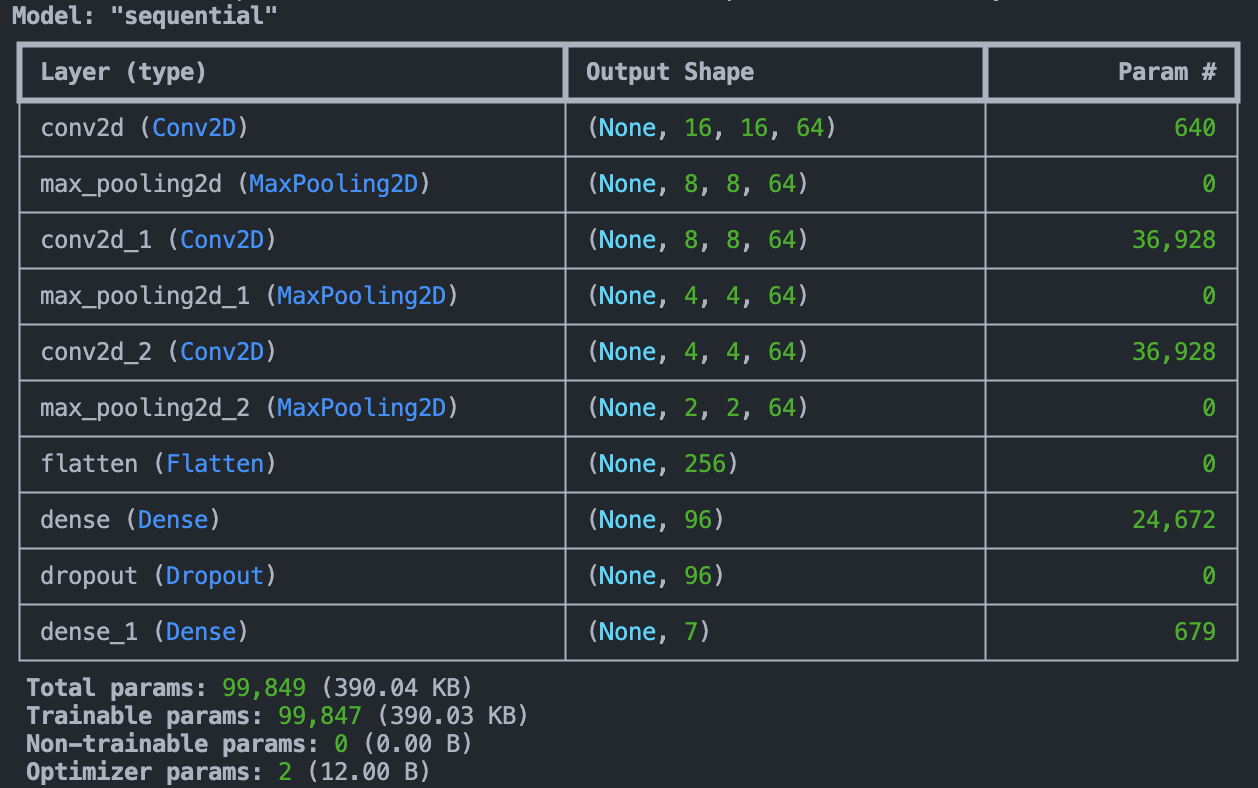
\includegraphics[width=0.8\linewidth]{images/cnn_architecture.png}
        \caption{Architettura del modello di CNN ottenuto} 
        \label{fig:cnn_architecture} 
    \end{figure}
    \newpage
    
    \item \textbf{Creazione della GAN}: Durante questa fase, è stata sviluppata una Generative Adversarial Network (GAN) per la generazione di nuovi campioni di malware. La GAN è stata progettata per apprendere le caratteristiche dei campioni di malware e generare nuovi esemplari che potessero essere utilizzati per ulteriori esperimenti e analisi. Il generatore della GAN crea immagini partendo da un vettore di rumore, mentre il discriminatore valuta la verosimiglianza delle immagini generate confrontandole con campioni autentici.

    L'approccio innovativo adottato permette non solo di arricchire il dataset con nuovi esempi, ma anche di testare la robustezza del modello di classificazione preaddestrato. Attraverso un processo iterativo di manipolazione delle immagini, si cerca di ingannare il modello. Ogni immagine è manipolata fino a dieci volte, registrando le metriche di successo e il numero di iterazioni per ciascuna prova. Questo processo è eseguito in parallelo mediante l'uso del \textit{ThreadPoolExecutor}, migliorando significativamente l'efficienza computazionale.

    Inoltre, vengono generati grafici per ciascuna categoria di malware, mostrando la relazione tra il numero di iterazioni di manipolazione e la precisione del modello. Questi grafici, salvati automaticamente, servono per valutare visivamente l'efficacia della GAN nel creare campioni che mettano alla prova il modello di classificazione.

    L'architettura specifica della GAN include dettagli sui layer del generatore e del discriminatore. Si discute l'efficacia del modello nel generare immagini che siano innovativi e utili per ulteriori analisi di sicurezza, includendo una discussione sull'addestramento della GAN e le strategie per bilanciare la competizione tra generatore e discriminatore, assicurando che il generatore non produca campioni troppo facili da classificare o troppo distanti dai veri esempi di malware.

    \item \textbf{Esperimenti}: Sono stati condotti esperimenti per valutare l'efficacia della rete neurale convoluzionale (CNN) e della GAN. Le prestazioni della rete neurale sono state misurate in termini di accuratezza e precisione nella classificazione dei malware, mentre la qualità dei campioni generati dalla GAN è stata valutata in base alla loro somiglianza con i campioni reali. \textit{[Aggiungere informazioni sui risultati ottenuti, metodi di valutazione utilizzati, ecc.]}
    
    \item \textbf{Analisi dei Risultati}: In questa fase, sono stati analizzati i risultati ottenuti dagli esperimenti. L'analisi si è concentrata sulla valutazione della capacità del modello di classificare correttamente i malware e sulla qualità dei malware generati dalla GAN. È stata inoltre eseguita una valutazione qualitativa dei risultati per identificare eventuali limiti del modello e miglioramenti possibili.
    
    \item \textbf{Conclusioni}: Al termine degli esperimenti e dell'analisi, sono state tratte le conclusioni finali riguardo l'efficacia delle tecniche utilizzate e i risultati ottenuti. Sono state inoltre discusse le potenzialità future del progetto, le aree di miglioramento e le implicazioni per l'analisi automatica e la generazione di malware.
\end{enumerate}


\subsection{Tecnologie Specifiche per GAN}
~\\
\indent Per la realizzazione della componente blackbox all'interno della GAN, è stata utilizzata la libreria Keras di TensorFlow, uno strumento potente e flessibile per la costruzione di modelli di deep learning, disponibile per Python. Keras facilita l'implementazione di reti neurali complesse attraverso un'interfaccia di alto livello e modulare.

Il modello di rete neurale convoluzionale (CNN) è stato sviluppato completamente da zero, addestrando un dataset appositamente creato e classificato dal tirocinante. Per la costruzione della GAN, invece, si è fatto riferimento a architetture di modelli avanzati e già validati come MalGAN, Xception e Inception, che sono noti per la loro elevata precisione e robustezza.

In particolare:
\begin{itemize}
    \item \textbf{MalGAN} ha dimostrato un'elevata efficienza nel bypassare soluzioni antimalware basate su blackbox, raggiungendo un tasso di successo vicino al 99\% in alcuni scenari.
    \item \textbf{Xception}, che utilizza un approccio basato su moduli di separazione di convoluzioni profonde, ha mostrato una precisione notevole nella classificazione di immagini, superando altri modelli preesistenti.
    \item \textbf{Inception}, noto anche come GoogLeNet, è rinomato per la sua complessità e l'efficienza, essendo stato il vincitore della ImageNet Challenge nel 2014.
\end{itemize}

Queste tecnologie sono state integrate per sfruttare le loro capacità di generalizzazione e precisione, potenziando significativamente l'efficacia della GAN sviluppata.

\footnote{\url{https://keras.io/}}
\footnote{\url{https://www.tensorflow.org/}}
\footnote{\url{https://github.com/lzylucy/Malware-GAN-attack}}
\footnote{\url{https://arxiv.org/abs/1610.02357}}


% \subsection{Tecnologie Specifiche per Dataset}
% ~\\


\section{Esperimenti}
~\\
\indent La sezione corrente esamina in dettaglio gli esperimenti condotti nel corso dello studio, illustrando la logica sottostante e le procedure impiegate per la loro realizzazione. 
L'obiettivo è fornire una panoramica completa delle attività sperimentali, cosicchè ci sia una maggiore comprensione sia dei metodi utilizzati che degli scopi.
\\\\
Gli esperimenti sono stati creati con l'obiettivo di identificare e testare diversi metodi per aumentare la precisione nel riconoscimento dei malware.
\\\\
I relativi risultati vengono analizzati nel Capitolo \ref{cap:risultati} mentre le conclusioni raggiunte sono discusse nel Capitolo \ref{cap:conclusioni}.

\subsection{Esperimenti relativi a qualche tipo di GAN applicata}
~\\ 
%TODO aggiungere dettagli come per esempio la percentuale di riconoscimento delle famiglie di malware. 



% % QUESTA PARTE VA MESSA PER SPIEGARE DOPO LE COPPIE MNEMONICHE: 
% In particolare, dall'assembly si è scelto di considerare solo le istruzioni mnemoniche, ignorando qualsiasi altro tipo di dato. Questi mnemonici rappresentano le operazioni fondamentali svolte dal codice, fornendo una sintesi compatta e significativa del comportamento del malware. Dopo aver estratto i mnemonici, si sono generate tutte le possibili coppie di mnemonici, cioè sequenze di due istruzioni consecutive, per catturare le relazioni immediate tra le operazioni eseguite.

% Una volta ottenute le coppie di mnemonici, si è applicata la tecnica TF-IDF (Term Frequency - Inverse Document Frequency), che consente di quantificare l'importanza di ciascuna coppia nel contesto dell'intero dataset. L'uso di TF-IDF permette di ridurre l'influenza di coppie di mnemonici troppo comuni (meno informative) e di enfatizzare quelle che risultano particolarmente distintive per certe famiglie di malware.

% Dopo l'applicazione di TF-IDF, si è proceduto con una riduzione dimensionale utilizzando la PCA (Principal Component Analysis), selezionando i componenti principali che meglio rappresentano la variabilità nei dati. Questo ha consentito di ridurre la complessità delle informazioni mantenendo al contempo una buona rappresentazione delle caratteristiche distintive del malware.

% Dai componenti principali ottenuti, si è generata una matrice di dimensione 16x16, che rappresenta una sorta di "impronta" del comportamento del malware. Questa matrice è stata poi normalizzata utilizzando la tecnica Min-Max Scaling, che trasforma i valori della matrice in un range tra 0 e 255, permettendo così di rappresentarli come intensità di pixel.

% Infine, la matrice normalizzata è stata convertita in un'immagine in scala di grigi, dove ogni pixel rappresenta un valore numerico della matrice scalato tra 0 (nero) e 255 (bianco). Questo processo ha portato alla generazione di immagini di dimensione 16x16 pixel, che sono utilizzate come input per la rete neurale convoluzionale.